% Template LaTeX file for DAFx-25 papers
%
% To generate the correct references using BibTeX, run
%     latex, bibtex, latex, latex
% modified...
% - from DAFx-00 to DAFx-02 by Florian Keiler, 2002-07-08
% - from DAFx-03 to DAFx-04 by Gianpaolo Evangelista, 2004-02-07 
% - from DAFx-05 to DAFx-06 by Vincent Verfaille, 2006-02-05
% - from DAFx-06 to DAFx-07 by Vincent Verfaille, 2007-01-05
%                          and Sylvain Marchand, 2007-01-31
% - from DAFx-07 to DAFx-08 by Henri Penttinen, 2007-12-12
%                          and Jyri Pakarinen 2008-01-28
% - from DAFx-08 to DAFx-09 by Giorgio Prandi, Fabio Antonacci 2008-10-03
% - from DAFx-09 to DAFx-10 by Hannes Pomberger 2010-02-01
% - from DAFx-10 to DAFx-12 by Jez Wells 2011
% - from DAFx-12 to DAFx-14 by Sascha Disch 2013
% - from DAFx-15 to DAFx-16 by Pavel Rajmic 2015
% - from DAFx-16 to DAFx-17 by Brian Hamilton 2016
% - from DAFx-17 to DAFx-18 by Annibal Ferreira and Matthew Davies 2017
% - from DAFx-18 to DAFx-19 by Dave Moffat 2019
% - from DAFx-19 to DAFx-20-21-22 by Gianpaolo Evangelista 2019-21
% - from DAFx-20-21-22 to DAFx-23 by Federico Fontana 2022-11-25
% - from DAFx-23 to DAFx-24 by Matteo Scerbo 2023-10-05
% - from DAFx-24 to DAFx-25 by Leonardo Gabrielli 2024-12-13
%
% Template with hyper-references (links) active after conversion to pdf
% (with the distiller) or if compiled with pdflatex.
%
% 20060205: added package 'hypcap' to correct hyperlinks to figures and tables
%                      use of \papertitle and \paperauthorA, etc for same title in PDF and Metadata
% 20190205: Package 'hypcap' removed, and replaced with 'caption', to allow for the inclusion
%		       of a CC UP licence.
% 20221125: Package 'nimbusserif' commented. PDF test template generated with
%                      pdfTeX 3.14159265-2.6-1.40.20 (TeX Live 2019/Debian) kpathsea version 6.3.1
%
% 1) Please compile using latex or pdflatex.
% 2) If using pdflatex, you need your figures in a file format other than eps! e.g. png or jpg is working
% 3) Please use "paperftitle" and "pdfauthor" definitions below

%------------------------------------------------------------------------------------------
%  !  !  !  !  !  !  !  !  !  !  !  ! user defined variables  !  !  !  !  !  !  !  !  !  !  !  !  !  !
% Please use the following commands to define title and author(s) of the paper.
% paperauthorA MUST be the the first author of the paper
% Please comment the unused definitions 
\def\papertitle{Towards an objective comparison of panning feature algorithms for unsupervised learning}
\def\paperauthorA{Richard Mitic}
\def\paperauthorB{Andreas Rossholm}
% \def\paperauthorC{Author Three}
% \def\paperauthorD{Author Four}
%\def\paperauthorE{Author Five}
%\def\paperauthorF{Author Six}
%\def\paperauthorG{Author Seven}
%\def\paperauthorH{Author Eight}
%\def\paperauthorI{Author Nine}
%\def\paperauthorJ{Author Ten}

% Authors' affiliations have to be set below

%------------------------------------------------------------------------------------------
\documentclass[twoside,a4paper]{article}
\usepackage{etoolbox}
\usepackage{dafx_25}
\usepackage{amsmath,amssymb,amsfonts,amsthm}
\usepackage{euscript}
%\usepackage[latin1]{inputenc}
\usepackage[T1]{fontenc}
\usepackage[utf8]{inputenc}
%\usepackage[T1]{fontenc}
%\usepackage{lmodern}
%\usepackage{nimbusserif}
\usepackage{ifpdf}
\usepackage[british]{babel}
\usepackage{caption}
% \usepackage{subfig} % or can use subcaption package
\usepackage{subcaption}
\usepackage{color}
\usepackage{csquotes}
\usepackage{booktabs}
\usepackage{makecell}

% Vector notation should be bold and italic
\usepackage{bm}
\renewcommand{\vec}{\bm}

% Make tables easier to read
\renewcommand{\arraystretch}{1.4}

\usepackage{glossaries}
\makeglossary
\loadglsentries{glossary}

\input glyphtounicode
\pdfgentounicode=1

\setcounter{page}{1}
\ninept

% build the list of authors and set the flag \multipleauth to handle the et al. in the copyright note (in DAFx_24.sty)
%==============================DO NOT MODIFY =======================================
\newcounter{numauth}\setcounter{numauth}{1}
\newcounter{listcnt}\setcounter{listcnt}{1}
\newcommand\authcnt[1]{\ifdefined#1 \stepcounter{numauth} \fi}

\newcommand\addauth[1]{
\ifdefined#1 
\stepcounter{listcnt}
\ifnum \value{listcnt}<\value{numauth}
\appto\authorslist{, #1}
\else
\appto\authorslist{~and~#1}
\fi
\fi}
%======DO NOT MODIFY UNLESS YOUR PAPER HAS MORE THAN 10 AUTHORS========================
%==we count the authors defined at the beginning of the file (paperauthorA is mandatory and already accounted for)
\authcnt{\paperauthorB}
\authcnt{\paperauthorC}
\authcnt{\paperauthorD}
\authcnt{\paperauthorE}
\authcnt{\paperauthorF}
\authcnt{\paperauthorG}
\authcnt{\paperauthorH}
\authcnt{\paperauthorI}
\authcnt{\paperauthorJ}
%==we create a list of authors for pdf tagging, for example: paperauthorA, paperauthorB, ... and paperauthorF (last author)
\def\authorslist{\paperauthorA}
\addauth{\paperauthorB}
\addauth{\paperauthorC}
\addauth{\paperauthorD}
\addauth{\paperauthorE}
\addauth{\paperauthorF}
\addauth{\paperauthorG}
\addauth{\paperauthorH}
\addauth{\paperauthorI}
\addauth{\paperauthorJ}
%====================================================================================

\usepackage{times}
% Saves a lot of ouptut space in PDF... after conversion with the distiller
% Delete if you cannot get PS fonts working on your system.


% pdf-tex settings: detect automatically if run by latex or pdflatex
\newif\ifpdf
\ifx\pdfoutput\relax
\else
   \ifcase\pdfoutput
      \pdffalse
   \else
      \pdftrue
   \fi
\fi

\ifpdf % compiling with pdflatex
  \usepackage[pdftex,
    pdftitle={\papertitle},
    pdfauthor={\authorslist},
    pdfsubject={Proceedings of the 28th International Conference on Digital Audio Effects (DAFx25)},
    colorlinks=false, % links are activated as color boxes instead of color text
    bookmarksnumbered, % use section numbers with bookmarks
    pdfstartview=XYZ % start with zoom=100% instead of full screen; especially useful if working with a big screen :-)
  ]{hyperref}
  \pdfcompresslevel=9
  \usepackage[pdftex]{graphicx}
 % \usepackage[figure,table]{hypcap}
\else % compiling with latex
  \usepackage[dvips]{epsfig,graphicx}
  \usepackage[dvips,
    pdftitle={\papertitle},
    pdfauthor={\authorslist},
    pdfsubject={Proceedings of the 28th International Conference on Digital Audio Effects (DAFx25)},
    colorlinks=false, % no color links
    bookmarksnumbered, % use section numbers with bookmarks
    pdfstartview=XYZ % start with zoom=100% instead of full screen
  ]{hyperref}
  % hyperrefs are active in the pdf file after conversion
  %\usepackage[figure,table]{hypcap}
\fi
\usepackage[hypcap=true]{caption}
\title{\papertitle}

% Must load cleveref after hyperref
\usepackage{cleveref}

% Make all references short
\Crefname{equation}{Eq.}{Eqs.}
\Crefname{figure}{Fig.}{Figs.}
\Crefname{tabular}{Tab.}{Tabs.}

%-------------SINGLE-AFFILIATION SINGLE-AUTHOR HEADER STARTS (uncomment below if your paper has a single author)----------------------------------------
% \affiliation{
% \paperauthorA \,\sthanks{This work was supported by the KKS Foundation}}
% {\href{https://www.mdu.se/en/malardalen-university/about-mdu/organisation/school-of-innovation-design-and-g}{School of Innovation, Design and Engineering} \\ Mälardalens Universitet \\ Västerås, SE\\
% {\tt \href{mailto:richard.mitic@mdu.se}{richard.mitic@mdu.se}}
% }
%
%Please note that the copyright notice should be separated from the text by a line (like a footnote). This works automatically when you have an \sthanks command 
%in the authors' line. However, if your paper does not require an \sthanks command, please use an empty (vertical space eating) \thanks command as follows:
% \affiliation{
% \paperauthorA\,\thanks{\vspace{-3mm}}}
% {\href{https://dafx25.dii.univpm.it/}{Dept. of Information Engineering} \\ Universit\`a Politecnica delle Marche \\ Ancona, IT\\
% {\tt \href{mailto:dafx25@dii.univpm.it}{dafx25@dii.univpm.it}}
% }
%-------------SINGLE-AFFILIATION SINGLE-AUTHOR HEADER ENDS-------------------------------------------------------------------------------------------------------------------

%------------SINGLE-AFFILIATION MULTIPLE-AUTHORS HEADER STARTS (uncomment below if your paper has two or more authors from the same institution)
% \affiliation{
% \paperauthorA\,\sthanks{Thanks to the predecessors for the templates}and \paperauthorB \,\sthanks{This work was supported by the XYZ Foundation}}
% {\href{https://dafx25.dii.univpm.it/}{Dept. of Information Engineering} \\ Universit\`a Politecnica delle Marche \\ Ancona, IT\\
% {\tt \href{mailto:dafx25@dii.univpm.it}{dafx25@dii.univpm.it}}
% }
%
%Please note that the copyright notice should be separated from the text by a line (like a footnote). This works automatically when you have an \sthanks command 
%in the authors' line. However, if your paper does not require an \sthanks command, please use an empty (vertical space eating) \thanks command as follows:
% \affiliation{
% \paperauthorA\ and \paperauthorB\,\thanks{\vspace{-3mm}}}
% {\href{https://dafx25.dii.univpm.it/}{Dept. of Information Engineering} \\ Universit\`a Politecnica delle Marche \\ Ancona, IT\\
% {\tt \href{mailto:dafx25@dii.univpm.it}{dafx25@dii.univpm.it}}
% }
%-----------------------------------SINGLE-AFFILIATION-MULTIPLE-AUTHORS HEADER ENDS----------------------------------------------------------------------------------------

%---------------TWO-AFFILIATIONS HEADER STARTS (uncomment below if your paper has two authors, each from a different institution)-----------------------------
\twoaffiliations{
\paperauthorA \,\sthanks{This work was supported by the KKS Foundation}}
{\href{https://www.mdu.se/en/malardalen-university/about-mdu/organisation/school-of-innovation-design-and-g}{School of Innovation, Design and Engineering} \\ Mälardalens Universitet \\ Västerås, SE\\
{\tt \href{mailto:richard.mitic@mdu.se}{richard.mitic@mdu.se}}
}
{\paperauthorB}
{\href{https://spotify.com}{Spotify} \\ Stockholm, SE\\
{\tt \href{mailto:arossholm@spotify.com}{arossholm@spotify.com}}
}
% 
% Please note that the copyright notice should be separated from the text by a line (like a footnote). This works automatically when you have an \sthanks command 
% in the authors' line. However, if your paper does not require any \sthanks command, please use an empty (vertical space eating) \thanks command only in one of the authors
% headers as follows:
% \twoaffiliations{
% \paperauthorA \,\sthanks{Thanks to the predecessors for the templates}}
% {\href{https://dafx25.dii.univpm.it/}{Dept. of Information Engineering} \\ Universit\`a Politecnica delle Marche \\ Ancona, IT\\
% {\tt \href{mailto:dafx25@dii.univpm.it}{dafx25@dii.univpm.it}}
% }
% {\paperauthorB \,\sthanks{This work was supported by the XYZ Foundation}}
% {\href{https://dafx24.surrey.ac.uk}{Institute of Sound Recording} \\ University of Surrey\\ Guildford, UK\\
% {\tt \href{mailto:dafx24@surrey.ac.uk}{dafx24@surrey.ac.uk}}
% }
%-------------------------------------TWO-AFFILIATIONS HEADER ENDS------------------------------------------------------

%%---------------THREE-AFFILIATIONS HEADER STARTS (uncomment below if your paper has three authors, each from a different institution)-----------------------
% \threeaffiliations{
% \paperauthorA \,\sthanks{Thanks to the predecessors for the templates}}
% {\href{https://dafx25.dii.univpm.it/}{Dept. of Information Engineering} \\ Universit\`a Politecnica delle Marche \\ Ancona, IT\\
% {\tt \href{mailto:dafx25@dii.univpm.it}{dafx25@dii.univpm.it}}
% }
% {\paperauthorB \,\sthanks{This work was supported by the XYZ Foundation}}
% {\href{https://dafx24.surrey.ac.uk}{Institute of Sound Recording} \\ University of Surrey\\ Guildford, UK\\
% {\tt \href{mailto:dafx24@surrey.ac.uk}{dafx24@surrey.ac.uk}}
% }
% {\paperauthorC \,\sthanks{Illustrious contributor}}
% {\href{https://dafx23.create.aau.dk/}{Multisensory Experience Lab} \\ Aalborg University \\ Copenhagen, Denmark \\
% {\tt \href{mailto:dafx2023@gmail.com}{dafx2023@gmail.com}}
% }
%
%Please note that the copyright notice should be separated from the text by a line (like a footnote). This works automatically when you have an \sthanks command 
%in the authors' line. However, if your paper does not require any \sthanks command, please use an empty (vertical space eating) \thanks command only in one of the authors
%headers as follows:
% \threeaffiliations{
% \paperauthorA \,\sthanks{Thanks to the predecessors for the templates}}
% {\href{https://dafx25.dii.univpm.it/}{Dept. of Information Engineering} \\ Universit\`a Politecnica delle Marche \\ Ancona, IT\\
% {\tt \href{mailto:dafx25@dii.univpm.it}{dafx25@dii.univpm.it}}
% }
% {\paperauthorB \,\sthanks{This work was supported by the XYZ Foundation}}
% {\href{https://dafx24.surrey.ac.uk}{Institute of Sound Recording} \\ University of Surrey\\ Guildford, UK\\
% {\tt \href{mailto:dafx24@surrey.ac.uk}{dafx24@surrey.ac.uk}}
% }
% {\paperauthorC \,\sthanks{Illustrious contributor}}
% {\href{https://dafx23.create.aau.dk/}{Multisensory Experience Lab} \\ Aalborg University \\ Copenhagen, Denmark \\
% {\tt \href{mailto:dafx2023@gmail.com}{dafx2023@gmail.com}}
% }
%-------------------------------------THREE-AFFILIATIONS HEADER ENDS------------------------------------------------------

%----------------FOUR-AFFILIATIONS HEADER STARTS (uncomment below if your paper has four authors, each from a different institution)-----------------------
%  \fouraffiliations{
%  \paperauthorA \,\sthanks{Thanks to the predecessors for the templates}}
%  {\href{https://dafx25.dii.univpm.it/}{Dept. of Information Engineering} \\ Universit\`a Politecnica delle Marche \\ Ancona, IT\\
%  {\tt \href{mailto:dafx25@dii.univpm.it}{dafx25@dii.univpm.it}}
%  }
%  {\paperauthorB \,\sthanks{This work was supported by the XYZ Foundation}}
%  {\href{https://dafx24.surrey.ac.uk}{Institute of Sound Recording} \\ University of Surrey\\ Guildford, UK\\
%  {\tt \href{mailto:dafx24@surrey.ac.uk}{dafx24@surrey.ac.uk}}
%  }
%  {\paperauthorC \,\sthanks{Illustrious contributor}}
%  {\href{https://dafx23.create.aau.dk/}{Multisensory Experience Lab} \\ Aalborg University \\ Copenhagen, Denmark \\
%  {\tt \href{mailto:dafx2023@gmail.com}{dafx2023@gmail.com}}
%  }
%  {\paperauthorD \,\sthanks{This guy is a very good fellow}}
%  {\href{https://www.mdw.ac.at/ike/}{MDW} \\ University of Music and Performing Arts\\ Vienna, Austria\\
%  {\tt \href{mailto:dafx2022@gmail.com}{dafx2022@gmail.com}}
%  }
%
%Please note that the copyright notice should be separated from the text by a line (like a footnote). This works automatically when you have an \sthanks command 
%in the authors' line. However, if your paper does not require any \sthanks command, please use an empty (vertical space eating) \thanks command only in one of the authors
%headers as follows:
% \fouraffiliations{
% \paperauthorA \,\sthanks{Thanks to the predecessors for the templates}}
% {\href{https://dafx25.dii.univpm.it/}{Dept. of Information Engineering} \\ Universit\`a Politecnica delle Marche \\ Ancona, IT\\
% {\tt \href{mailto:dafx25@dii.univpm.it}{dafx25@dii.univpm.it}}
% }
% {\paperauthorB \,\sthanks{This work was supported by the XYZ Foundation}}
% {\href{https://dafx24.surrey.ac.uk}{Institute of Sound Recording} \\ University of Surrey\\ Guildford, UK\\
% {\tt \href{mailto:dafx24@surrey.ac.uk}{dafx24@surrey.ac.uk}}
% }
% {\paperauthorC \,\sthanks{Illustrious contributor}}
% {\href{https://dafx23.create.aau.dk/}{Multisensory Experience Lab} \\ Aalborg University \\ Copenhagen, Denmark \\
% {\tt \href{mailto:dafx2023@gmail.com}{dafx2023@gmail.com}}
% }
% {\paperauthorD \,\sthanks{This guy is a very good fellow}}
% {\href{https://www.mdw.ac.at/ike/}{MDW} \\ University of Music and Performing Arts\\ Vienna, Austria\\
% {\tt \href{mailto:dafx2022@gmail.com}{dafx2022@gmail.com}}
% }
%-------------------------------------FOUR-AFFILIATIONS HEADER ENDS------------------------------------------------------


% Names of tracks
\newcommand{\RM}{\textit{\gls{rm}}}
\newcommand{\TITT}{\textit{\gls{titt}}}
\newcommand{\LB}{\textit{\gls{lb}}}
\newcommand{\M}{\textit{\gls{m}}}
\newcommand{\CAC}{\textit{\gls{cac}}} 
\newcommand{\FMTTM}{\textit{\gls{fmttm}}}
\newcommand{\ISHST}{\textit{\gls{ishst}}}

\begin{document}
% more pdf-tex settings:
\ifpdf % used graphic file format for pdflatex
  \DeclareGraphicsExtensions{.png,.jpg,.pdf}
\else  % used graphic file format for latex
  \DeclareGraphicsExtensions{.eps}
\fi

%\makeatletter
%\pdfbookmark[0]{\@pdftitle}{title}
%\makeatother

\maketitle

\begin{abstract}
Estimations of panning attributes are an important feature to extract from a piece of recorded music, with downstream uses such as classification, quality assessment, and listening enhancement. While several algorithms exist in the literature, there is currently no comparison between them and no studies to suggest which one is most suitable for any particular task. This paper compares four algorithms for extracting amplitude panning features with respect to their suitability for unsupervised learning. It finds synchronicities between them and analyses their results on a small set of commercial music excerpts chosen for their distinct panning features. The ability of each algorithm to differentiate between the tracks is analysed. The results can be used in future work to either select the most appropriate panning feature algorithm or create a version customized for a particular task.
\end{abstract}

\section{Introduction}
\label{sec:intro}
The vast majority of recorded music available today was recorded and produced in stereophonic format. The musicians and producers involved will often pay close attention to the placement of sound objects in the stereo field, and various pieces of equipment such as goniometers, phase scopes, and stereo balance indicators have been standard equipment in recording studios for decades. There is therefore a wealth of spatial information encoded in the final recording. Extracting and disentangling that information has been the subject of research for many years, in various different guises. 

A typical use case is classification, where stereo features have been used as a predictor of genre \cite{tzanetakisStereoPanningFeatures2007,tzanetakisStereoPanningInformation2010,ziemerGoniometersArePowerful2023}, artist/composer/DJ \cite{tzanetakisStereoPanningInformation2010,ziemerAcousticFeaturesRecording2021}, and decade \cite{tardieuProductionEffectAudio2011}. Additionally, panning features have been used on their own merit (as opposed to predictors of another feature) for tasks such as source separation \cite{barrySoundSourceSeparation2004,shim2009Stereo}, upmixing \cite{avendano2002frequency}, and music similarity/recommendation \cite{gomezMusicSimilaritySystems2008,ziemerAcousticFeaturesRecording2021}. The classification of panning features themselves has also been studied as a precursor to upmixing, source separation, and audio enhancement \cite{harmaStereoAudioClassification2011,harmaClassificationTimefrequencyRegions2011}, giving the ability to select appropriate algorithms based on audio content.

In the aforementioned cases, the audio analysed has either comprised single excerpts or lists of 1000-2000 tracks with labels assigned. However, in recent years much bigger musical datasets have become available, e.g. \cite{bogdanovMTGJamendoDatasetAutomatic2019,fma_dataset}, which contain 55000 and 100000 tracks respectively. These datasets do not contain any metadata regarding panning features, nor any similar information such as recording methods/style. While they do offer genre and date tags, panning features on their own have previously shown low correlation with genre and decade \cite{tzanetakisStereoPanningInformation2010,tardieuProductionEffectAudio2011}, from which we can infer that genre and date cannot be reliably used a proxy for panning features. If one wishes to use these datasets for the aforementioned use cases, there is hence a need to perform unsupervised learning on the extracted panning features, and for this to be successful we must understand the abilities and limits of the extraction method being used. 

Several examples of panning feature extractors for stereo audio signals exist in the literature \cite{tzanetakisStereoPanningFeatures2007,sarroffMeasurementsSpaciousnessStereophonic2008,gomezMusicSimilaritySystems2008,tardieuProductionEffectAudio2011}, but as yet there has not been a comparison of them and no discussion of what panning features they are able to detect. The aim of this paper is to provide such discussion. It will begin by summarizing the relevant literature in \Cref{sec:previouswork}, describing and drawing links between existing panning feature extraction algorithms. \Cref{sec:method} presents examples of commercial music chosen for their different uses of amplitude panning, plus the methods used to compare the panning feature algorithms. \Cref{sec:results} shows the results of the analysis and \Cref{sec:discussion} will discuss some overall trends that emerged across all algorithms. Concluding remarks are offered in \Cref{sec:conclusion}.

\section{Previous work}
\label{sec:previouswork}

\cite{avendano2002frequency,avendanoFrequencydomainSourceIdentification2003} are seminal works describing the \enquote{panning index} -- a description of amplitude panning for each time-frequency bin in a stereo spectrogram. \cite{avendano2002frequency} also presents the \enquote{ambience index} -- a measure of inter-channel correlation in \gls{tf} bins. While they target re-synthesis and upmix as use cases, the underlying techniques have become the basis for many applications since. 
\cite{barrySoundSourceSeparation2004} is another seminal work which describes a frequency-azimuth plane constructed from phase cancellation of delayed stereo \gls{tf} planes. Similarly, it targets re-panning and re-synthesis but has since been repurposed.
\cite{tzanetakisStereoPanningFeatures2007,tzanetakisStereoPanningInformation2010} reuse the panning index from \cite{avendano2002frequency} (renamed to \enquote{\gls{sps}}) and derive a set of \gls{spf} that are used for genre classification and \gls{mir}.
\cite{sarroffMeasurementsSpaciousnessStereophonic2008} details a method to estimate the perceptual stereo width of a music recording by forming a \gls{ph} based on the frequency-azimuth plane from \cite{barrySoundSourceSeparation2004}.
Another \gls{ph} method (this time based on the \gls{sps} from \cite{tzanetakisStereoPanningFeatures2007}) is described in \cite{gomezMusicSimilaritySystems2008,guausAudioContentProcessing2009}, specifying the measurement of music similarity as the primary use case. It contributes an extra step of converting the \gls{ph} into \gls{pc} through cepstral analysis, stating that this allows the resulting vector to be used with any generic classification algorithm.
In a similar vein (and with classification as a use case) \cite{tardieuProductionEffectAudio2011} combines cochleagram differences with an analysis of phase differences between channels to form two feature sets - the \enquote{\gls{asf}} and \enquote{\gls{psf}}.

\cite{harmaClassificationTimefrequencyRegions2010,harmaClassificationTimefrequencyRegions2011,harmaStereoAudioClassification2011} collectively define a new paradigm of classifying regions of audio whereby stereo mixtures are modelled as combinations of centre, panned, and uncorrelated sources. Even though genre classification is used as an example use case, they specifically state that the class representing a combination of all source types (i.e. most music recordings) is very difficult to identify and therefore omitted from the model.

Similar to the phase-based features defined in \cite{tardieuProductionEffectAudio2011}, there are a group of algorithms based on the emulation of a studio goniometer; \cite{ziemerAcousticFeaturesRecording2021,ziemerGoniometersArePowerful2023} use both a goniometer box-counting technique and inter-channel correlation analysis to derive a time-varying measurement of \enquote{spaciousness}. Interestingly though, \cite{stirnatSpaciousnessMusicTonmeisters2019} found that subjective impressions of spaciousness in various musical styles were largely contradictory to the results of goniometer analysis.

More recently, \gls{ml}-based techniques for disentangling spatial information from audio content have been demonstrated. With a primary use case of upmixing stereo to multichannel, \cite{yangUpmixingStyleTransfer2022} demonstrates that a latent vector formed by running multichannel audio through one half of the learned neural network represents the spatial information contained in the original signal. Similarly, \cite{yangSelfSupervisedLearningSpatial2024a} takes a stereo microphone input and regenerates one channel from the other by learning an inter-channel spatial representation. Mirroring our problem statement, \cite{yangSelfSupervisedLearningSpatial2024a} specifically mentions a lack of labelled real-world data as motivation for the use of unsupervised learning.

\subsection{Selected algorithms}
\label{ssec:selectedalgorithms}
This paper will focus on four algorithms that estimate panning features from stereophonic commercial music recordings and do not require training on a dataset. Specifically,  \gls{ph} \cite{sarroffMeasurementsSpaciousnessStereophonic2008} \gls{pc} \cite{gomezMusicSimilaritySystems2008}, \gls{asf} \cite{tardieuProductionEffectAudio2011}, and \gls{spf} \cite{tzanetakisStereoPanningFeatures2007}. For mathematical definitions the reader is referred to the original papers, but a summary of each is given here.

\subsubsection{\acrfull{ph} --- Sarroff, 2008 \cite{sarroffMeasurementsSpaciousnessStereophonic2008}}
The left and right channels are split into chunks and transformed into the frequency domain using a \gls{fft}. Each \gls{fft} frame is converted into a \gls{fa} plane through phase cancellation techniques. The left and right \gls{fa} planes are concatenated, and a histogram is calculated across all frames and all frequencies. The result is a histogram of energy at each azimuth bin.

Note: The paper continues to collapse the histogram into a single scalar representing overall width, but we will not consider that here since the intent is to compare the \gls{ph} vector with other high-dimensional representations of panning features.

\subsubsection{\acrfull{pc} --- Gomez, 2008 \cite{gomezMusicSimilaritySystems2008}}
The left and right channels are split into chunks and transformed into magnitude spectrograms using a \gls{stft}. The ratio of power spectra is calculated for each frame, resulting in an azimuthal panning factor each frequency bin. These values are warped by a function that accounts for the human perception of the direction of arrival of sounds. Each frame is then converted to an energy-weighted histogram and the mean over time is taken. The histogram is then converted to a compact representation by performing cepstral analysis and truncating the results to length 20.

\subsubsection{\acrfull{asf} --- Tardieu, 2011 \cite{tardieuProductionEffectAudio2011}}
The \gls{asf} are created from a stereo cochleagram. Left and right audio channels are split into frequency sub-bands using gammatone filters spaced equally on the \gls{erb} scale. The amplitude difference of the two cochleagram channels is taken to produce a \gls{cd}. The \glspl{asf} are created by taking the mean and standard deviation over various axes of the \gls{cd}. The mathematical definition of a cochleagram is not given in \cite{tardieuProductionEffectAudio2011}, so for this paper we have followed the steps in \cite{isobeRelationshipsInterauralCrosscorrelation2012}, creating a cochleagram directly from time domain audio as opposed to using an \gls{fft}. \cite{tardieuProductionEffectAudio2011} also does not state the exact form of the resulting vector, so for this paper all features are simply concatenated into a single vector.

\subsubsection{\acrfull{spf} --- Tzanetakis, 2007 \cite{tzanetakisStereoPanningFeatures2007}}
The left and right channels are converted into complex \gls{tf} regions by chunking, windowing, and the \gls{stft}. These two \gls{tf} regions are converted into an \gls{sps}, which is then split into high, mid, and low frequency bands. Each sub-band (along with the full spectrum) are collapsed by calculating the \gls{rms} across the frequency dimension, and smoothed in time by calculating a running mean and standard deviation over $M$ frames. The mean and standard deviation over time are then calculated, resulting in a 16-dimensional vector.

\section{Method}
\label{sec:method}

To assess each algorithm they are run on a selection of musical excerpts exhibiting panning features that it would be useful to differentiate between. As a way of delineating the entire panning feature gamut, we use two \enquote{anchor tracks} - one strongly mono and one strongly stereo. The other tracks each represent an interesting panning feature. For each algorithm, the panning features for all tracks are calculated and considered to be points in an N-dimensional feature space. The Euclidean distances ($D$) between pairs of tracks are calculated, and the set for each algorithm is normalized so that $D \in [0,1]$. Specifically, it is hypothesized that 

\begin{enumerate}
  \item The anchor tracks should be located farthest apart in the feature space \label{hyp:anchors}
  \item The panning feature tracks should be well separated and evenly distributed between the anchors \label{hyp:sep}
\end{enumerate}

Any pair with low separation (i.e. the algorithm cannot differentiate between them) is further examined to find out why. We define a low separation to be $D<0.1$. 

\subsection{Musical excerpts}
\label{ssec:method_musical_excerpts}

All excerpts are defined by their title, artist, release year, and timing information. For the rest of the paper they will be referred to by abbreviated title. The panning features they exhibit are also defined here. Anchor tracks are denoted by \enquote{*} for mono and \enquote{**} for stereo.

\begin{itemize}
  \item \RM{}, Miles Davis, 1957, 0:00--0:30. A jazz piece recorded in mono.
  \item \TITT{}, Fink, 2007, 1:00--1:30. An acoustic song with studio reverb added. The vocal switches from single-tracked to multi-tracked with moderate amplitude\linebreak panning approximately halfway though the excerpt.
  \item \LB{}, Low, 2001, 0:00--0:30. Electric guitar, bass, and vocals with an enveloping sound created mostly by reverberation and multi-miking, but only subtle amplitude panning.
  \item \M{}, Chilly Gonzales, 2025, 1:00--1:30. Solo upright piano recorded live on stage with close stereo microphones. Individual notes are audibly separated in space even though no studio panning has been applied.
  \item \CAC{}, Tetsu Inoue, 2000, 0:00--0:30. An electronic piece that is characterized by heavy use of extreme panning, unnatural sounds, and singular audio events with very short durations.
  \item \FMTTM{}, Frank Sinatra, 2008, 1:00--1:30. A full big band recorded live. Most instruments are statically panned to a fairly strong degree.
  \item \ISHST{}, The Beatles, 1963, 0:00--0:30. A pop song with strong, rudimentary panning. Drums, bass, and lead guitar are panned hard left, while vocals and rhythm guitar are panned hard right.
\end{itemize}

We define \enquote{natural panning} to mean that recorded instruments that have been amplitude panned to a static position in the final recording. Examples of natural panning are \TITT{}, \FMTTM{}, and \ISHST{}. The counterpart is \enquote{unnatural panning}, which we use to refer to sounds that move very fast between left and right. \CAC{} is an example of unnatural panning. 

All recordings have a sample rate $f_s=44100$ Hz and were normalized to an average loudness of -23 \gls{lufs} before processing according to \cite{ebu-r-128LoudnessNormalisationPermitted2023,itu-r-bs.1770-4AlgorithmsMeasureAudio2015}.

\subsection{Algorithm parameters}
Each algorithm is defined by a set of input parameters, and the values used for this paper are shown in \Cref{tab:algorithm_parameters}. For precise meanings of each one, the reader is directed to the original papers.


\begin{table}[htbp]
  \renewcommand{\arraystretch}{1.4}
  \begin{tabular}{p{0.2\columnwidth} p{0.44\columnwidth} p{0.16\columnwidth}}
    \toprule
    Algorithm & Parameters & Dimensions \\
    \midrule
    \acrshort{ph} \cite{sarroffMeasurementsSpaciousnessStereophonic2008} & \makecell[lt]{FFT size = 1024 \\ hop size = 512 \\ azimuth bins = 129}  & 129 \\
    \acrshort{pc} \cite{gomezMusicSimilaritySystems2008} & \makecell[lt]{FFT size = 1024 \\ hop size = 512 \\ azimuth bins = 129 \\  cepstrum coefficients = 20} & 20 \\
    \acrshort{asf} \cite{tardieuProductionEffectAudio2011} & \makecell[lt]{Low $f_c$ = 30Hz \\ High $f_c$ = 11050Hz \\ number of bands = 70 \\ chunk length = 20ms \\ hop length = 10ms} & 272 \\
    \acrshort{spf} \cite{tzanetakisStereoPanningFeatures2007} & \makecell[lt]{FFT size = 1024 \\ hop size = 512 \\ M = 40 \\ low band = 0-250 Hz \\ mid band = 250-2500 Hz \\ high band = 2500-22050 Hz } & 16 \\
    \bottomrule
  \end{tabular}
  \caption{\it Parameters for panning algorithms \label{tab:algorithm_parameters}}
\end{table}


\section{Results}
\label{sec:results}

\begin{figure*}[htbp!]
  \centering
  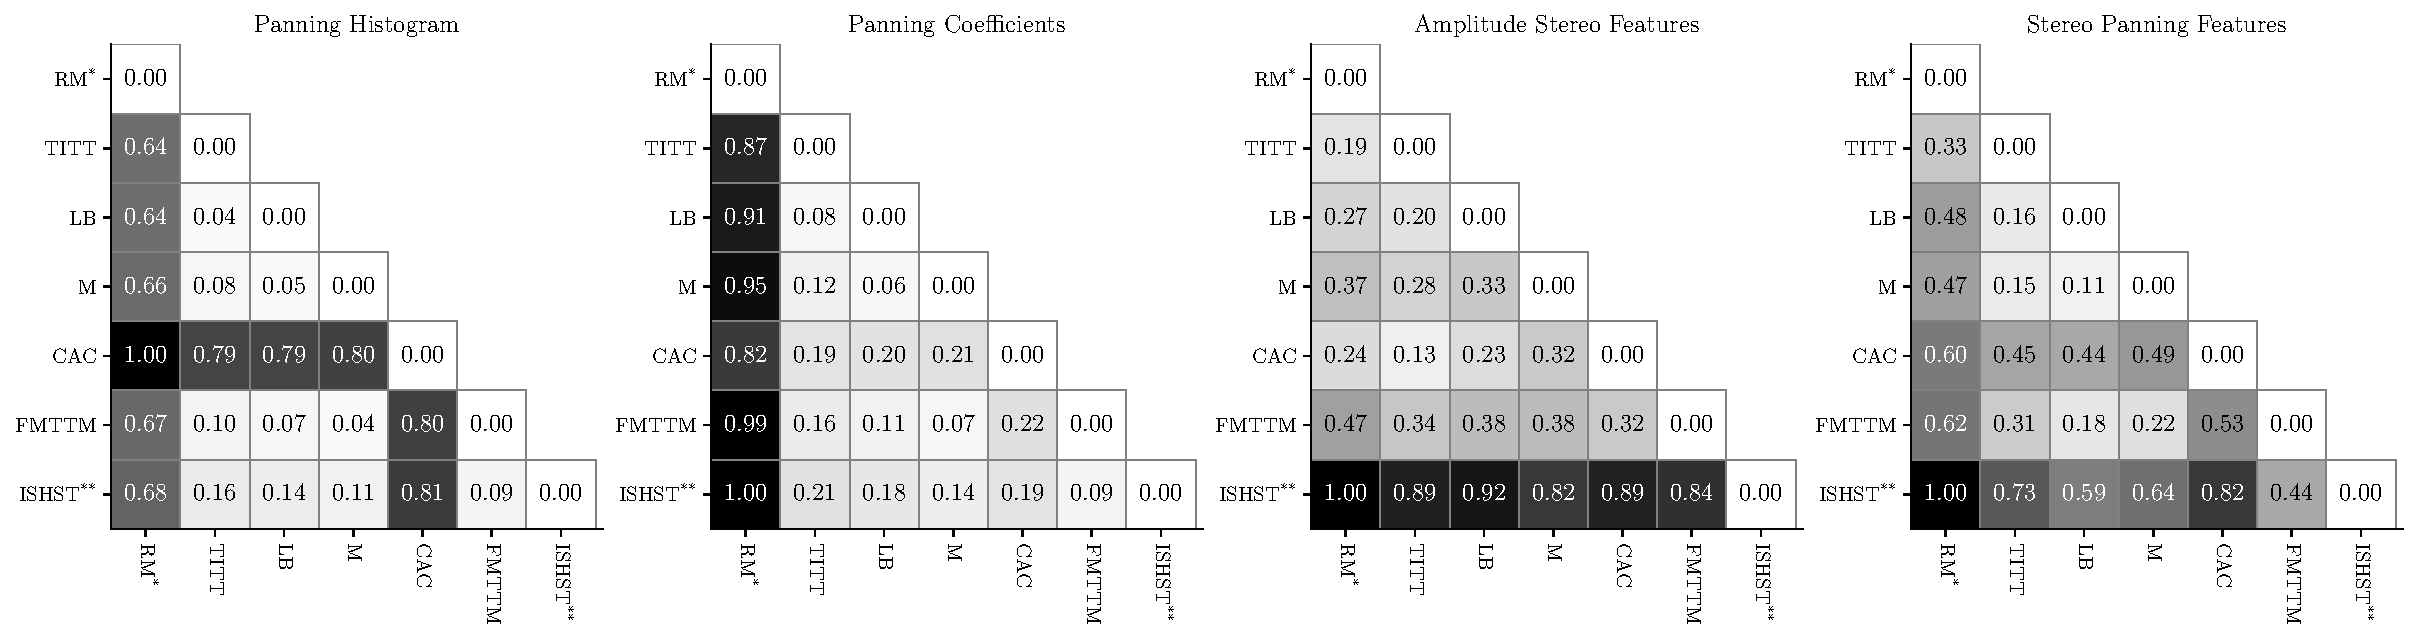
\includegraphics[width=\textwidth]{sip_images/distance_matrices.pdf}
  \caption{{\it Distance between pairs of tracks in the feature spaces of the four panning feature algorithms. \label{fig:distance_matrices}}}
\end{figure*}

The Euclidean distances between pairs of tracks in each feature space are shown in \Cref{fig:distance_matrices}. Within each feature space, distances have been normalized to the range $D \in [0,1]$. Cells are coloured in greyscale with white and black representing 0 and 1 respectively, and track titles are abreviated.

\Cref{fig:distance_matrices} shows that some panning feature algorithms have a clear bias towards one of the anchor tracks. (visible as a much darker section in otherwise pale matrix). A bias towards the mono anchor (i.e. a dark horizontal line on the bottom row) means that all panning feature tracks appear \enquote{very mono} to the algorithm. Conversely, a bias towards the stereo anchor (i.e. a dark vertical line in the left column) means that all panning feature tracks appear as \enquote{very stereo} to the algorithm.

To quantify this, we define a \enquote{bias score} ($B$) according to \Cref{eq:bias_score}. Firstly the mean distances from each anchor track to all panning feature tracks are calculated, then $B$ is defined as the natural logarithm of the ratio of mean mono distance ($\bar{D}_m$) to mean stereo distance ($\bar{D}_s$). A score of $B=0$ means no bias, a positive score ($B>0$) means a bias towards the stereo anchor and negative score ($B<0$) means a bias towards the mono anchor. This is calculated by \Cref{eq:bias_score} where $T = \{ t : t \in T \}$ is the set of panning feature tracks, $D_{m,t}$ is the distance between the mono anchor and a panning feature track, and $D_{s,t}$ is the distance between the stereo anchor and a panning feature track.

\begin{equation}
  \label{eq:bias_score}
  \begin{split}
    \bar{D}_m &= \frac{1}{|T|} \sum_{t \in T} D_{m,t} \\
    \bar{D}_s &= \frac{1}{|T|} \sum_{t \in T} D_{s,t} \\
    B &= \ln\frac{\bar{D}_m}{\bar{D}_s}
  \end{split}
\end{equation}

The scores for each algorithm are shown in \Cref{tab:anchor_distances} alongside their interpretations. 

\begin{table}[h]
  \centering
  \begin{tabular}{lcccl}
    \toprule
    Algorithm & $\bar{D}_m$ & $\bar{D}_s$ & $B$ & Interpretation \\
    \midrule
    \gls{ph} \cite{sarroffMeasurementsSpaciousnessStereophonic2008} & 0.72 & 0.26 & 1.02 & strong stereo bias \\
    \gls{pc} \cite{gomezMusicSimilaritySystems2008} & 0.91 & 0.16 & 1.73 & very strong stereo bias \\
    \gls{asf} \cite{tardieuProductionEffectAudio2011} & 0.31 & 0.87 & -1.04 & strong mono bias \\
    \gls{spf} \cite{tzanetakisStereoPanningFeatures2007} & 0.50 & 0.64 & -0.25 & slight mono bias \\
    \bottomrule
  \end{tabular}
  \caption{\it Bias scores for all panning feature algorithms \label{tab:anchor_distances}} 
\end{table}

From \Cref{fig:distance_matrices} it is simple to test hypothesis \ref{hyp:anchors} (the anchor tracks should be the furthest apart) by finding the cell with a value of 1. It is also possible to assess hypothesis \ref{hyp:sep} (the other tracks should be well separated) by finding cells with low values. Each panning feature algorithm will be assessed separately.

% \newpage

\subsection{\acrlong{ph} \cite{sarroffSpaciousnessRecordedMusic2009}}
\label{sec:results_ph}
\Cref{fig:distance_matrices} shows that this is the only algorithm for which hypothesis \ref{hyp:anchors} is not satisfied. Instead of the two anchor tracks (\RM{} and \ISHST{}) having the largest distance, \RM{} and \CAC{} are in fact the two most separated tracks. To determine why this was the case, the \glspl{ph} of all three tracks are plotted in \Cref{fig:ph_cut_round}. 

\begin{figure}[htbp]
  \centering
  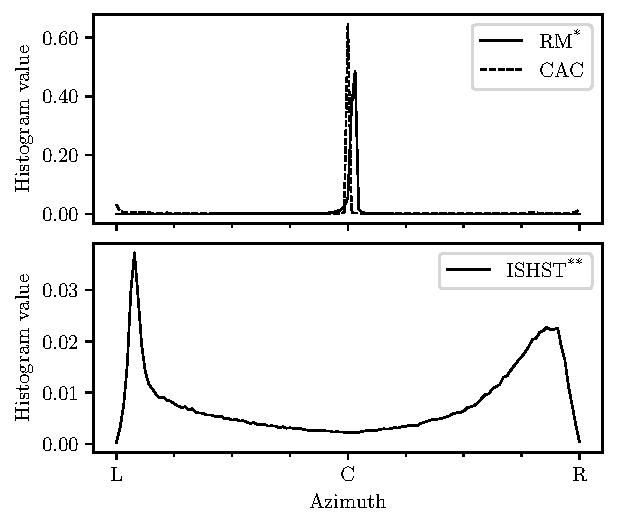
\includegraphics[width=\columnwidth]{sip_images/ph_rm_cac_ishst_overlay.pdf}
  \caption{\it \acrshortpl{ph} of \RM{}, \CAC{} and \ISHST{}, demonstrating that \CAC{} has been wrongly detected as monophonic. \label{fig:ph_cut_round}}
\end{figure}

\begin{figure}[htbp]
  \centering
  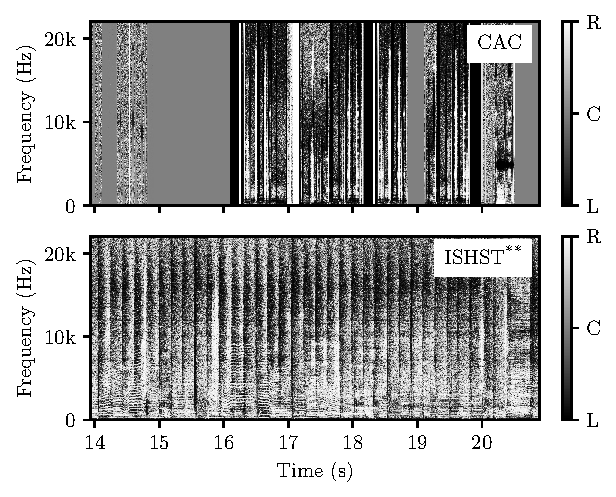
\includegraphics[width=\columnwidth]{sip_images/sps_cac_ishst.pdf}
  \caption{\it \acrlong{sps} of a short section of \CAC{} and \ISHST{}. \label{fig:ph_cuts_panning_spect}}
\end{figure}

From this diagram we can observe two important phenomena. Firstly, \CAC{} (which is characterized by extreme and unnatural panning) actually appears close to mono in its \gls{ph}. By inspecting the panning spectrogram (a section of which is shown in \Cref{fig:ph_cuts_panning_spect}) we see that when hard panning occurs, \acrlong{tf} frames panned hard left and right are roughly evenly distributed. Hence, when the mean over time is taken, the hard-panned frames cancel each other out and all energy appears to be located in the centre. This differs from e.g. \ISHST{} which consistently has energy panned to both channels simultaneously and hence has two histogram peaks on the left and right. 

Secondly, even though \RM{} and \CAC{} have similarly-shaped \acrshortpl{ph}, their Euclidean distance is very large. This is because the central peaks of each track appear in different azimuth bins. Since each bin is a separate dimension in the feature space, these two tracks effectively appear as two vectors with large amplitudes pointing in different directions. From this we can determine that the Euclidean distance is not a good measure of similarity for \acrlongpl{ph}, and we will therefore not assess hypothesis \ref{hyp:sep}.

\subsection{\acrlong{pc} \cite{gomezMusicSimilaritySystems2008}}
\label{sec:results_pc}
Inspection of \Cref{fig:distance_matrices} reveals that, as hypothesized, \RM{} and \ISHST{} are the two tracks with the most separation. However, as \Cref{tab:anchor_distances} shows, it also has a strong bias towards the stereo anchor. The tracks \TITT{}, \LB{}, \M{}, and \FMTTM{} all appear in close pairs, implying that \gls{pc} might have trouble differentiating between tracks that use moderate, but different, amplitude panning techniques. Reassuringly though, tracks that include extreme panning are separated from moderately-panned tracks, with $D \approx 0.2$.

The \gls{pc} algorithm is based on a \acrlong{ph} that is quantized by truncation in the cepstral domain. To assess the effect of this, we can reverse the cepstral process using \Cref{eq:reverse_cepstrum} where $\vec{c}$ is the vector of cepstral coefficients that has been truncated to length $L$. First, a pseudo-spectrum $\vec{s}$ is created by taking the exponential of the real part of the \gls{dft} of $\vec{c}$. $\vec{s}$ is then truncated to half its length to recreate a histogram, and normalized so that the total area is 1. The result is a \acrlong{ph} $\vec{h}$ with $L/2$ azimuth bins.

\begin{equation}
  \label{eq:reverse_cepstrum}
  \begin{split}
    \vec{c} & = (c_1, c_2, \dots{} ,c_L) \\ 
    \vec{s} &= \exp(\text{Re}(\text{DFT}(\vec{c}))) \\
    \vec{h} &= \frac{\vec{s}_{1:L/2}}{\frac{L}{2} \sum \vec{s}_{1:L/2}}
  \end{split}
\end{equation}


\Cref{fig:phc_quant} shows the quantized and original \glspl{ph} for \ISHST{} and its three closest neighbours. From these diagrams it is clear to see why the \gls{pc} algorithm is biased towards the stereo anchor - the anchor itself has had its panning energy moved from the side lobes towards the centre, and hence the detected panning features are more akin to the moderately-panned tracks (which are not so affected by the quantization). 

\begin{figure}[htbp]
  \centering
  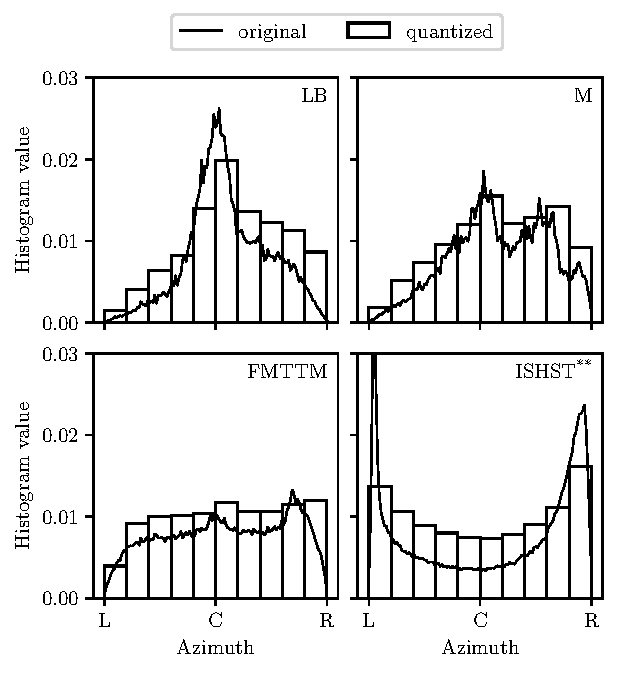
\includegraphics[width=\linewidth]{sip_images/phc_quant_4.pdf}
  \caption{\it \glspl{ph} of \ISHST{} and its three closest neighbours before and after cepstral quantization.\label{fig:phc_quant}}
\end{figure}


\subsection{\acrlong{asf} \cite{tardieuProductionEffectAudio2011}}
\label{sec:results_asf}
Similarly to \gls{pc}, the \gls{asf} distance matrix (\Cref{fig:distance_matrices}) shows that the two anchor tracks are indeed the furthest separated. Conversely though, \Cref{tab:anchor_distances} shows that \gls{asf} has a bias towards the mono anchor. The separation of all tracks except \ISHST{} is, however, quite adequate, with a range of $D \in [0.13, 0.47]$.

Curiously, \FMTTM{} and \ISHST{} have a high separation ($D=0.84$) despite both exhibiting strong natural panning. \Cref{fig:asf_fmttm_ishst} shows a visual representation of \gls{asf} for these two tracks. The panning features \enquote{mean over time} and \enquote{standard deviation over time} (see \cite{tardieuProductionEffectAudio2011}) for each cochlea band are depicted as dots with error bars. From this diagram it is clear the two tracks have roughly opposite panning along the frequency axis. For example, \FMTTM{} has a double bass panned to the right, while \ISHST{} has a bass guitar panned to the left. This difference in panning direction is certainly a contributor to the high separation between these two tracks, and hence the overall mono bias of \gls{asf}.

\begin{figure}[t]
  \centering
  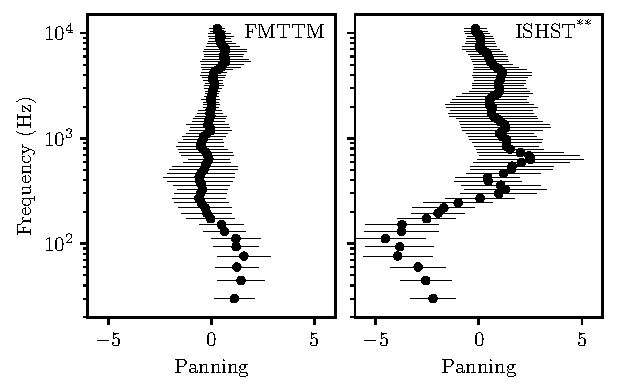
\includegraphics[width=\columnwidth]{sip_images/asf_fmttm_ishst.pdf}
  \caption{\it \gls{asf} for \FMTTM{} and \ISHST{} showing similar frequency bands panned in opposite directions.\label{fig:asf_fmttm_ishst}}
\end{figure}

It is also notable that the panning variation for both tracks shown in \Cref{fig:asf_fmttm_ishst} is quite high, when we can hear in the original audio that instruments are panned statically. This is most likely caused by overlapping frequency components in the left and right spectra -- a common issue discussed in previous literature \cite{avendano2002frequency,barrySoundSourceSeparation2004,fitzgeraldInpaintingAdressAlgorithm2012}. Certainly the phenomenon is not unique to the \gls{asf} algorithm but nevertheless is illustrated particularly well by this diagram.

\begin{figure}[b]
  \centering
  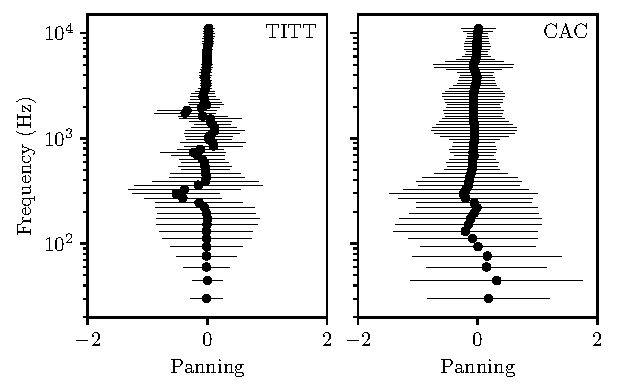
\includegraphics[width=\columnwidth]{sip_images/asf_titt_cac.pdf}
  \caption{\it \gls{asf} for \TITT{} and \CAC{}, both exhibiting average central panning. \label{fig:asf_titt_cac}}
\end{figure}

\begin{figure}[htb]
  \centering
  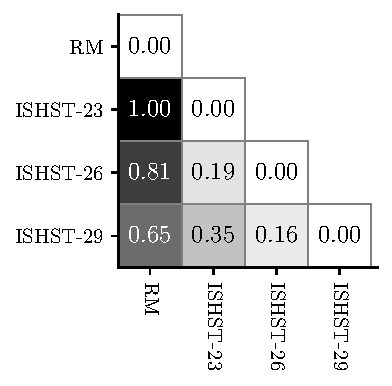
\includegraphics[width=0.5\columnwidth]{sip_images/distance_matrix_different_lufs.pdf}
  \caption{\it Distance matrix comparing \RM{} (at -23 \gls{lufs}) to \ISHST{} at -23, -26, and -29 \gls{lufs}.\label{fig:asf_different_gains}}
\end{figure}

While not too close by our standards, \CAC{} and \TITT{} ($D=0.13$) are the closest pair. This is surprising since one would imagine that the moderate, natural panning of \TITT{} would be well separated from the extreme, unnatural panning of \CAC{}. Examining their \gls{asf} plots (see \Cref{fig:asf_titt_cac}) reveals that while the panning variation of each track is quite different, they both exhibit mean panning that is roughly centred, mirroring the \gls{ph} error described in \Cref{sec:results_ph}. One possible explanation is that the fast panning of \CAC{} manifests more as phase difference than amplitude difference, which would match the dispersion introduced by the reverberation in \TITT{}. While panning variation for \CAC{} is much higher in the lower frequencies, it could be the case that the high number of dimensions in \gls{asf} is acting to quash those differences.

One important factor in the use of \gls{asf} is that its calculation (defined in \cite{tardieuProductionEffectAudio2011}) does not include any step to account for the overall loudness of the audio. To demonstrate the effect of this, we can calculate another distance matrix comparing \RM{} to several versions of \ISHST{} that are normalized to different loudness levels. \Cref{fig:asf_different_gains} visualizes this and clearly shows that the relative loudness of two tracks affects their distance in the feature space. All tracks analysed in this paper were normalized to equal loudness to account for this, but that might not be possible in a real-world use case, e.g. analysing streaming audio in real time.


\subsection{\acrlong{spf} \cite{tzanetakisStereoPanningFeatures2007}}
\label{sec:results_spf}
The distance matrix (\Cref{fig:distance_matrices}) for \gls{spf} reveals that the two anchor tracks are indeed the furthest separated, and \Cref{tab:anchor_distances} shows the lowest bias. There are also no track pairs with a low separation. However, the distance matrix does show a generally high separation for \CAC{}. This implies that \gls{spf} is able to differentiate between natural and unnatural panning quite well. In particular, \CAC{} is maximally separated from \ISHST{} even though both contain extreme panning. 

The definition of \gls{spf} includes estimations of both \enquote{short-term panning} (the running standard deviation over $M$ frames) and \enquote{long-term panning} (the running mean over $M$ frames). These are calculated over four frequency bands (fullband, lows, mids, and highs), and the global means and standard deviations of these comprise the final feature vector. We can therefore visualize the \gls{spf} as a scatter plot with the vertical position of a point denoting the amount of panning in each frequency band and error bars denoting panning variation, with short- and long-term values separated. 

\Cref{fig:spf_cac_ishst} shows the \gls{spf} plots for \CAC{} alongside the two anchor tracks. It reveals that indeed, the unnatural panning of \CAC{} is visible as large error bars in all dimensions whereas \ISHST{} has much higher average panning and relatively low variation, thus demonstrating how \gls{spf} is able to differentiate between natural and unnatural panning.

\begin{figure}[htbp]
  \centering
  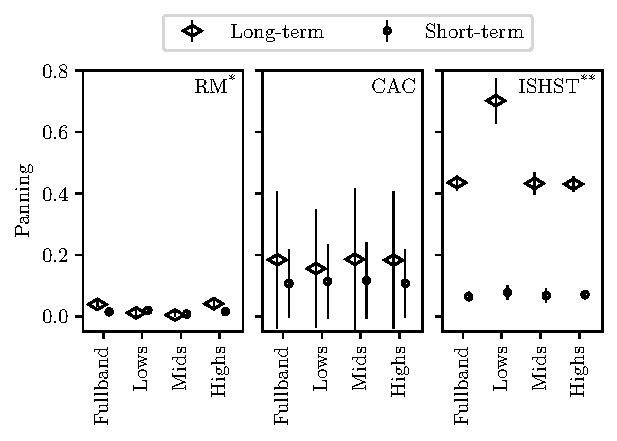
\includegraphics[width=\columnwidth]{sip_images/spf_rm_cac_ishst.pdf}
  \caption{\it \gls{spf} plots for \RM{}, \CAC{} and \ISHST{} showing clear separation between all three.\label{fig:spf_cac_ishst}}
\end{figure}

\RM{} has low, but non-negligible values in all dimensions. Inspection of the original formula \cite{tzanetakisStereoPanningFeatures2007} shows that a truly mono signal would produce an \gls{spf} vector of all 0s, revealing that \RM{} is, in fact, not entirely mono. By listening to the difference between the left and right channels, we can hear that the original mono recording has had a decorrelation effect applied at the mastering stage. We can therefore conclude that \gls{spf} is sensitive to this kind of effect.

\begin{table*}[htb]
  \renewcommand{\arraystretch}{1.618} % Make the table really easy to read
  \centering
\begin{tabular}{p{0.06\linewidth} p{0.14\linewidth} p{0.07\linewidth} p{0.07\linewidth} p{0.08\linewidth} p{0.08\linewidth} p{0.32\linewidth}}
\toprule
Algorithm & Frequency bands & Variation over time & Panning direction & Azimuthal resolution & Loudness invariant & Notes \\
\midrule
\gls{ph} \cite{sarroffMeasurementsSpaciousnessStereophonic2008} & Fullband & No & Yes & High & Yes & \makecell[lt]{Cannot use Euclidean distance.\\Azimuthal resolution configurable.}\\
\gls{pc} \cite{gomezMusicSimilaritySystems2008} & Fullband & No & Yes & Low & Yes & \makecell[lt]{Strong stereo details are lost.\\Azimuthal resolution configurable.}\\
\gls{asf} \cite{tardieuProductionEffectAudio2011} & \gls{erb}, 70 bands & Yes & Yes & High & No & \makecell[lt]{Strong mono bias.\\Very large feature space.}\\
\gls{spf} \cite{tzanetakisStereoPanningFeatures2007} & Lows, Mids, Highs & Yes & No & High & Yes & \makecell[lt]{Relatively low bias.\\Separates natural/unnatural panning well.\\Sensitive to decorrelation effects.}\\
\bottomrule
\end{tabular}
  \caption{\it Summary of properties for all panning feature algorithms.\label{tab:aglo_summary}}
\end{table*}

% \pagebreak
\section{Discussion}
\label{sec:discussion}

\Cref{tab:aglo_summary} shows a summary of each algorithm. For the purposes of unsupervised learning on commercial music, \gls{spf} has shown the most promise as it has the lowest bias score and good separation between all the panning feature tracks. The features related to panning variation over time appear to be important as they can help avoid issues such as the misidentification of unnatural panning as monophonic audio (see \Cref{sec:results_ph}).

Each algorithm explicitly chooses whether to represent the panning \emph{direction} or just the panning \emph{amount}. \gls{asf} even includes features for both. Likewise, some algorithms act on frequency sub-bands whereas others process the entire spectrum. When the intention is to use panning features for unsupervised learning, the importance of both panning direction and frequency sub-bands is application-specific; any of the algorithms could be modified to include or exclude these two features.

The computational complexity of the algorithms was not addressed in this paper, but varied significantly among them. \gls{sps}-based descriptors (\cite{tzanetakisStereoPanningFeatures2007,gomezMusicSimilaritySystems2008}) are reliant on an \gls{stft} for their \gls{tf} representation and hence are efficient but sometimes difficult to reconcile with human perception, whereas algorithms based on cochleagrams (\cite{tardieuProductionEffectAudio2011}) produce more perceptually relevant results but require very large banks of time-domain filters.

An additional variable not covered by this paper is the duration of analysis. For the purposes of this experiment, 30s was chosen to roughly match \cite{tzanetakisStereoPanningFeatures2007}, although \cite{gomezMusicSimilaritySystems2008} mentions that any duration between 2s and the entire recording is acceptable and \cite{tardieuProductionEffectAudio2011} shows examples of entire songs. 


All algorithms differ greatly in the number of dimensions represented in the final panning features. When calculating Euclidean distances in N-dimensional space, it has been proven that the inclusion of variables which provide no additional accuracy both increases the distance between points and raises the likelihood of attributing significance to spurious measurements \cite{thireyDistributionEuclideanDistances2015}. A balance must therefore be struck between the resolution of the panning features and the ease of differentiating between tracks. Again, each algorithm can be modified to increase or decrease the dimensionality. 

% \pagebreak
\section{Conclusion}
\label{sec:conclusion}
Four panning feature extraction algorithms were tested with respect to their use for unsupervised learning. They were run on five tracks that exhibit interesting panning features, plus two \enquote{strongly mono} and \enquote{strongly stereo} anchor tracks. The algorithms' results for individual tracks were analysed to assess what panning features each algorithm is able to differentiate between. Each algorithm was assigned a \enquote{bias score} based on how the panning feature tracks were distributed within the anchor tracks. \gls{spf} from \cite{tzanetakisStereoPanningFeatures2007} showed the most promise, although it lacks differentiation between left and right and has relatively low frequency resolution.

In future work using panning features for unsupervised learning we recommend setting precise requirements for relevant panning features and choosing an algorithm accordingly based on the results given here. Alternatively, algorithms may be modified or combined to suit a specific need. The inclusion of other spatial descriptors such as those based on phase differences or generated via \gls{ml} might also prove fruitful. To that end, a much larger survey of spatial analysis techniques would be beneficial. 

In the cases where the original literature performed experiments on a commercial music collection \cite{tzanetakisStereoPanningFeatures2007,tardieuProductionEffectAudio2011}, it is not possible to fully reproduce their results since the exact tracks are unspecified. Analysis of modern, open datasets (e.g. \cite{bogdanovMTGJamendoDatasetAutomatic2019,fma_dataset}) would therefore be advantageous and would strengthen the results obtained in the current experiments.


% \newpage
% \nocite{*}
\bibliographystyle{IEEEbib}
\bibliography{library}

\end{document}
